%%
% Copyright (c) 2017 - 2020, Pascal Wagler;
% Copyright (c) 2014 - 2020, John MacFarlane
%
% All rights reserved.
%
% Redistribution and use in source and binary forms, with or without
% modification, are permitted provided that the following conditions
% are met:
%
% - Redistributions of source code must retain the above copyright
% notice, this list of conditions and the following disclaimer.
%
% - Redistributions in binary form must reproduce the above copyright
% notice, this list of conditions and the following disclaimer in the
% documentation and/or other materials provided with the distribution.
%
% - Neither the name of John MacFarlane nor the names of other
% contributors may be used to endorse or promote products derived
% from this software without specific prior written permission.
%
% THIS SOFTWARE IS PROVIDED BY THE COPYRIGHT HOLDERS AND CONTRIBUTORS
% "AS IS" AND ANY EXPRESS OR IMPLIED WARRANTIES, INCLUDING, BUT NOT
% LIMITED TO, THE IMPLIED WARRANTIES OF MERCHANTABILITY AND FITNESS
% FOR A PARTICULAR PURPOSE ARE DISCLAIMED. IN NO EVENT SHALL THE
% COPYRIGHT OWNER OR CONTRIBUTORS BE LIABLE FOR ANY DIRECT, INDIRECT,
% INCIDENTAL, SPECIAL, EXEMPLARY, OR CONSEQUENTIAL DAMAGES (INCLUDING,
% BUT NOT LIMITED TO, PROCUREMENT OF SUBSTITUTE GOODS OR SERVICES;
% LOSS OF USE, DATA, OR PROFITS; OR BUSINESS INTERRUPTION) HOWEVER
% CAUSED AND ON ANY THEORY OF LIABILITY, WHETHER IN CONTRACT, STRICT
% LIABILITY, OR TORT (INCLUDING NEGLIGENCE OR OTHERWISE) ARISING IN
% ANY WAY OUT OF THE USE OF THIS SOFTWARE, EVEN IF ADVISED OF THE
% POSSIBILITY OF SUCH DAMAGE.
%%

%%
% This is the Eisvogel pandoc LaTeX template.
%
% For usage information and examples visit the official GitHub page:
% https://github.com/Wandmalfarbe/pandoc-latex-template
%%

% Options for packages loaded elsewhere
\PassOptionsToPackage{unicode}{hyperref}
\PassOptionsToPackage{hyphens}{url}
\PassOptionsToPackage{dvipsnames,svgnames*,x11names*,table}{xcolor}
%
\documentclass[
  12pt,
  english,
  a4paper,
,tablecaptionabove
]{scrartcl}
\usepackage{lmodern}
\usepackage{setspace}
\setstretch{1.5}
\usepackage{amssymb,amsmath}
\usepackage{ifxetex,ifluatex}
\ifnum 0\ifxetex 1\fi\ifluatex 1\fi=0 % if pdftex
  \usepackage[T1]{fontenc}
  \usepackage[utf8]{inputenc}
  \usepackage{textcomp} % provide euro and other symbols
\else % if luatex or xetex
  \usepackage{unicode-math}
  \defaultfontfeatures{Scale=MatchLowercase}
  \defaultfontfeatures[\rmfamily]{Ligatures=TeX,Scale=1}
\fi
% Use upquote if available, for straight quotes in verbatim environments
\IfFileExists{upquote.sty}{\usepackage{upquote}}{}
\IfFileExists{microtype.sty}{% use microtype if available
  \usepackage[]{microtype}
  \UseMicrotypeSet[protrusion]{basicmath} % disable protrusion for tt fonts
}{}
\makeatletter
\@ifundefined{KOMAClassName}{% if non-KOMA class
  \IfFileExists{parskip.sty}{%
    \usepackage{parskip}
  }{% else
    \setlength{\parindent}{0pt}
    \setlength{\parskip}{6pt plus 2pt minus 1pt}}
}{% if KOMA class
  \KOMAoptions{parskip=half}}
\makeatother
\usepackage{xcolor}
\definecolor{default-linkcolor}{HTML}{A50000}
\definecolor{default-filecolor}{HTML}{A50000}
\definecolor{default-citecolor}{HTML}{4077C0}
\definecolor{default-urlcolor}{HTML}{4077C0}
\IfFileExists{xurl.sty}{\usepackage{xurl}}{} % add URL line breaks if available
% load footmisc in order to customize footnotes (footmisc has to be loaded before hyperref, cf. https://tex.stackexchange.com/a/169124/144087)
\usepackage[hang,flushmargin,bottom,multiple]{footmisc}
\setlength{\footnotemargin}{0.8em} % set space between footnote nr and text
\setlength{\footnotesep}{\baselineskip} % set space between multiple footnotes
\setlength{\skip\footins}{0.3cm} % set space between page content and footnote
\setlength{\footskip}{0.9cm} % set space between footnote and page bottom
\IfFileExists{bookmark.sty}{\usepackage{bookmark}}{\usepackage{hyperref}}
\hypersetup{
  pdftitle={Efficiency of Univariate Kernel Density Estimation with TensorFlow},
  pdfauthor={Marc Steiner},
  pdflang={en},
  pdfkeywords={Kernel Density Estimation, Python, TensorFlow},
  hidelinks,
  breaklinks=true,
  pdfcreator={LaTeX via pandoc with the Eisvogel template}}
\urlstyle{same} % disable monospaced font for URLs
\usepackage[left=4cm, right=3cm, top=2.5cm, bottom=2.5cm]{geometry}
\usepackage[export]{adjustbox}
\usepackage{graphicx}
\usepackage{listings}
\newcommand{\passthrough}[1]{#1}
\lstset{defaultdialect=[5.3]Lua}
\lstset{defaultdialect=[x86masm]Assembler}
\usepackage{color}
\usepackage{fancyvrb}
\newcommand{\VerbBar}{|}
\newcommand{\VERB}{\Verb[commandchars=\\\{\}]}
\DefineVerbatimEnvironment{Highlighting}{Verbatim}{commandchars=\\\{\}}
% Add ',fontsize=\small' for more characters per line
\usepackage{framed}
\definecolor{shadecolor}{RGB}{248,248,248}
\newenvironment{Shaded}{\begin{snugshade}}{\end{snugshade}}
\newcommand{\AlertTok}[1]{\textcolor[rgb]{0.94,0.16,0.16}{#1}}
\newcommand{\AnnotationTok}[1]{\textcolor[rgb]{0.56,0.35,0.01}{\textbf{\textit{#1}}}}
\newcommand{\AttributeTok}[1]{\textcolor[rgb]{0.77,0.63,0.00}{#1}}
\newcommand{\BaseNTok}[1]{\textcolor[rgb]{0.00,0.00,0.81}{#1}}
\newcommand{\BuiltInTok}[1]{#1}
\newcommand{\CharTok}[1]{\textcolor[rgb]{0.31,0.60,0.02}{#1}}
\newcommand{\CommentTok}[1]{\textcolor[rgb]{0.56,0.35,0.01}{\textit{#1}}}
\newcommand{\CommentVarTok}[1]{\textcolor[rgb]{0.56,0.35,0.01}{\textbf{\textit{#1}}}}
\newcommand{\ConstantTok}[1]{\textcolor[rgb]{0.00,0.00,0.00}{#1}}
\newcommand{\ControlFlowTok}[1]{\textcolor[rgb]{0.13,0.29,0.53}{\textbf{#1}}}
\newcommand{\DataTypeTok}[1]{\textcolor[rgb]{0.13,0.29,0.53}{#1}}
\newcommand{\DecValTok}[1]{\textcolor[rgb]{0.00,0.00,0.81}{#1}}
\newcommand{\DocumentationTok}[1]{\textcolor[rgb]{0.56,0.35,0.01}{\textbf{\textit{#1}}}}
\newcommand{\ErrorTok}[1]{\textcolor[rgb]{0.64,0.00,0.00}{\textbf{#1}}}
\newcommand{\ExtensionTok}[1]{#1}
\newcommand{\FloatTok}[1]{\textcolor[rgb]{0.00,0.00,0.81}{#1}}
\newcommand{\FunctionTok}[1]{\textcolor[rgb]{0.00,0.00,0.00}{#1}}
\newcommand{\ImportTok}[1]{#1}
\newcommand{\InformationTok}[1]{\textcolor[rgb]{0.56,0.35,0.01}{\textbf{\textit{#1}}}}
\newcommand{\KeywordTok}[1]{\textcolor[rgb]{0.13,0.29,0.53}{\textbf{#1}}}
\newcommand{\NormalTok}[1]{#1}
\newcommand{\OperatorTok}[1]{\textcolor[rgb]{0.81,0.36,0.00}{\textbf{#1}}}
\newcommand{\OtherTok}[1]{\textcolor[rgb]{0.56,0.35,0.01}{#1}}
\newcommand{\PreprocessorTok}[1]{\textcolor[rgb]{0.56,0.35,0.01}{\textit{#1}}}
\newcommand{\RegionMarkerTok}[1]{#1}
\newcommand{\SpecialCharTok}[1]{\textcolor[rgb]{0.00,0.00,0.00}{#1}}
\newcommand{\SpecialStringTok}[1]{\textcolor[rgb]{0.31,0.60,0.02}{#1}}
\newcommand{\StringTok}[1]{\textcolor[rgb]{0.31,0.60,0.02}{#1}}
\newcommand{\VariableTok}[1]{\textcolor[rgb]{0.00,0.00,0.00}{#1}}
\newcommand{\VerbatimStringTok}[1]{\textcolor[rgb]{0.31,0.60,0.02}{#1}}
\newcommand{\WarningTok}[1]{\textcolor[rgb]{0.56,0.35,0.01}{\textbf{\textit{#1}}}}

% Workaround/bugfix from jannick0.
% See https://github.com/jgm/pandoc/issues/4302#issuecomment-360669013)
% or https://github.com/Wandmalfarbe/pandoc-latex-template/issues/2
%
% Redefine the verbatim environment 'Highlighting' to break long lines (with
% the help of fvextra). Redefinition is necessary because it is unlikely that
% pandoc includes fvextra in the default template.
\usepackage{fvextra}
\DefineVerbatimEnvironment{Highlighting}{Verbatim}{breaklines,fontsize=\small,commandchars=\\\{\}}

\usepackage{longtable,booktabs}
% Correct order of tables after \paragraph or \subparagraph
\usepackage{etoolbox}
\makeatletter
\patchcmd\longtable{\par}{\if@noskipsec\mbox{}\fi\par}{}{}
\makeatother
% Allow footnotes in longtable head/foot
\IfFileExists{footnotehyper.sty}{\usepackage{footnotehyper}}{\usepackage{footnote}}
\makesavenoteenv{longtable}
% add backlinks to footnote references, cf. https://tex.stackexchange.com/questions/302266/make-footnote-clickable-both-ways
\usepackage{footnotebackref}
\usepackage{graphicx}
\makeatletter
\def\maxwidth{\ifdim\Gin@nat@width>\linewidth\linewidth\else\Gin@nat@width\fi}
\def\maxheight{\ifdim\Gin@nat@height>\textheight\textheight\else\Gin@nat@height\fi}
\makeatother
% Scale images if necessary, so that they will not overflow the page
% margins by default, and it is still possible to overwrite the defaults
% using explicit options in \includegraphics[width, height, ...]{}
\setkeys{Gin}{width=\maxwidth,height=\maxheight,keepaspectratio}
\setlength{\emergencystretch}{3em}  % prevent overfull lines
\providecommand{\tightlist}{%
  \setlength{\itemsep}{0pt}\setlength{\parskip}{0pt}}
\setcounter{secnumdepth}{3}

% Make use of float-package and set default placement for figures to H.
% The option H means 'PUT IT HERE' (as  opposed to the standard h option which means 'You may put it here if you like').
\usepackage{float}
\floatplacement{figure}{H}

\usepackage{booktabs}
\ifxetex
    % See issue https://github.com/reutenauer/polyglossia/issues/127
  \renewcommand*\familydefault{\sfdefault}
    % Load polyglossia as late as possible: uses bidi with RTL langages (e.g. Hebrew, Arabic)
  \usepackage{polyglossia}
  \setmainlanguage[]{english}
\else
  \usepackage[shorthands=off,main=english]{babel}
\fi

\title{Efficiency of Univariate Kernel Density Estimation with TensorFlow\thanks{true}}
\usepackage{etoolbox}
\makeatletter
\providecommand{\subtitle}[1]{% add subtitle to \maketitle
  \apptocmd{\@title}{\par {\large #1 \par}}{}{}
}
\makeatother
\subtitle{Bachelor Thesis}
\author{Marc Steiner}
\date{}



%%
%% added
%%

%
% language specification
%
% If no language is specified, use English as the default main document language.
%



%
% for the background color of the title page
%
\usepackage{pagecolor}
\usepackage{afterpage}
\usepackage{tikz}

%
% break urls
%
\PassOptionsToPackage{hyphens}{url}

%
% When using babel or polyglossia with biblatex, loading csquotes is recommended
% to ensure that quoted texts are typeset according to the rules of your main language.
%
\usepackage{csquotes}

%
% captions
%
\definecolor{caption-color}{HTML}{777777}
\usepackage[font={stretch=1.2}, textfont={color=caption-color}, position=top, skip=4mm, labelfont=bf, singlelinecheck=false, justification=raggedright]{caption}
\setcapindent{0em}

%
% blockquote
%
\definecolor{blockquote-border}{RGB}{221,221,221}
\definecolor{blockquote-text}{RGB}{119,119,119}
\usepackage{mdframed}
\newmdenv[rightline=false,bottomline=false,topline=false,linewidth=3pt,linecolor=blockquote-border,skipabove=\parskip]{customblockquote}
\renewenvironment{quote}{\begin{customblockquote}\list{}{\rightmargin=0em\leftmargin=0em}%
\item\relax\color{blockquote-text}\ignorespaces}{\unskip\unskip\endlist\end{customblockquote}}

%
% Source Sans Pro as the de­fault font fam­ily
% Source Code Pro for monospace text
%
% 'default' option sets the default
% font family to Source Sans Pro, not \sfdefault.
%
\ifnum 0\ifxetex 1\fi\ifluatex 1\fi=0 % if pdftex
    \usepackage[default]{sourcesanspro}
  \usepackage{sourcecodepro}
  \else % if not pdftex
    \usepackage[default]{sourcesanspro}
  \usepackage{sourcecodepro}

  % XeLaTeX specific adjustments for straight quotes: https://tex.stackexchange.com/a/354887
  % This issue is already fixed (see https://github.com/silkeh/latex-sourcecodepro/pull/5) but the
  % fix is still unreleased.
  % TODO: Remove this workaround when the new version of sourcecodepro is released on CTAN.
  \ifxetex
    \makeatletter
    \defaultfontfeatures[\ttfamily]
      { Numbers   = \sourcecodepro@figurestyle,
        Scale     = \SourceCodePro@scale,
        Extension = .otf }
    \setmonofont
      [ UprightFont    = *-\sourcecodepro@regstyle,
        ItalicFont     = *-\sourcecodepro@regstyle It,
        BoldFont       = *-\sourcecodepro@boldstyle,
        BoldItalicFont = *-\sourcecodepro@boldstyle It ]
      {SourceCodePro}
    \makeatother
  \fi
  \fi

%
% heading color
%
\definecolor{heading-color}{RGB}{40,40,40}
\addtokomafont{section}{\color{heading-color}}
% When using the classes report, scrreprt, book,
% scrbook or memoir, uncomment the following line.
%\addtokomafont{chapter}{\color{heading-color}}

%
% variables for title and author
%
\usepackage{titling}
\title{Efficiency of Univariate Kernel Density Estimation with TensorFlow}
\author{Marc Steiner}

%
% tables
%

\definecolor{table-row-color}{HTML}{F5F5F5}
\definecolor{table-rule-color}{HTML}{999999}

%\arrayrulecolor{black!40}
\arrayrulecolor{table-rule-color}     % color of \toprule, \midrule, \bottomrule
\setlength\heavyrulewidth{0.3ex}      % thickness of \toprule, \bottomrule
\renewcommand{\arraystretch}{1.3}     % spacing (padding)


%
% remove paragraph indention
%
\setlength{\parindent}{0pt}
\setlength{\parskip}{6pt plus 2pt minus 1pt}
\setlength{\emergencystretch}{3em}  % prevent overfull lines

%
%
% Listings
%
%


%
% general listing colors
%
\definecolor{listing-background}{HTML}{F7F7F7}
\definecolor{listing-rule}{HTML}{B3B2B3}
\definecolor{listing-numbers}{HTML}{B3B2B3}
\definecolor{listing-text-color}{HTML}{000000}
\definecolor{listing-keyword}{HTML}{435489}
\definecolor{listing-keyword-2}{HTML}{1284CA} % additional keywords
\definecolor{listing-keyword-3}{HTML}{9137CB} % additional keywords
\definecolor{listing-identifier}{HTML}{435489}
\definecolor{listing-string}{HTML}{00999A}
\definecolor{listing-comment}{HTML}{8E8E8E}

\lstdefinestyle{eisvogel_listing_style}{
  language         = java,
  numbers          = left,
  xleftmargin      = 2.7em,
  framexleftmargin = 2.5em,
  backgroundcolor  = \color{listing-background},
  basicstyle       = \color{listing-text-color}\linespread{1.0}\small\ttfamily{},
  breaklines       = true,
  frame            = single,
  framesep         = 0.19em,
  rulecolor        = \color{listing-rule},
  frameround       = ffff,
  tabsize          = 4,
  numberstyle      = \color{listing-numbers},
  aboveskip        = 1.0em,
  belowskip        = 0.1em,
  abovecaptionskip = 0em,
  belowcaptionskip = 1.0em,
  keywordstyle     = {\color{listing-keyword}\bfseries},
  keywordstyle     = {[2]\color{listing-keyword-2}\bfseries},
  keywordstyle     = {[3]\color{listing-keyword-3}\bfseries\itshape},
  sensitive        = true,
  identifierstyle  = \color{listing-identifier},
  commentstyle     = \color{listing-comment},
  stringstyle      = \color{listing-string},
  showstringspaces = false,
  escapeinside     = {/*@}{@*/}, % Allow LaTeX inside these special comments
  literate         =
  {á}{{\'a}}1 {é}{{\'e}}1 {í}{{\'i}}1 {ó}{{\'o}}1 {ú}{{\'u}}1
  {Á}{{\'A}}1 {É}{{\'E}}1 {Í}{{\'I}}1 {Ó}{{\'O}}1 {Ú}{{\'U}}1
  {à}{{\`a}}1 {è}{{\'e}}1 {ì}{{\`i}}1 {ò}{{\`o}}1 {ù}{{\`u}}1
  {À}{{\`A}}1 {È}{{\'E}}1 {Ì}{{\`I}}1 {Ò}{{\`O}}1 {Ù}{{\`U}}1
  {ä}{{\"a}}1 {ë}{{\"e}}1 {ï}{{\"i}}1 {ö}{{\"o}}1 {ü}{{\"u}}1
  {Ä}{{\"A}}1 {Ë}{{\"E}}1 {Ï}{{\"I}}1 {Ö}{{\"O}}1 {Ü}{{\"U}}1
  {â}{{\^a}}1 {ê}{{\^e}}1 {î}{{\^i}}1 {ô}{{\^o}}1 {û}{{\^u}}1
  {Â}{{\^A}}1 {Ê}{{\^E}}1 {Î}{{\^I}}1 {Ô}{{\^O}}1 {Û}{{\^U}}1
  {œ}{{\oe}}1 {Œ}{{\OE}}1 {æ}{{\ae}}1 {Æ}{{\AE}}1 {ß}{{\ss}}1
  {ç}{{\c c}}1 {Ç}{{\c C}}1 {ø}{{\o}}1 {å}{{\r a}}1 {Å}{{\r A}}1
  {€}{{\EUR}}1 {£}{{\pounds}}1 {«}{{\guillemotleft}}1
  {»}{{\guillemotright}}1 {ñ}{{\~n}}1 {Ñ}{{\~N}}1 {¿}{{?`}}1
  {…}{{\ldots}}1 {≥}{{>=}}1 {≤}{{<=}}1 {„}{{\glqq}}1 {“}{{\grqq}}1
  {”}{{''}}1
}
\lstset{style=eisvogel_listing_style}

%
% Java (Java SE 12, 2019-06-22)
%
\lstdefinelanguage{Java}{
  morekeywords={
    % normal keywords (without data types)
    abstract,assert,break,case,catch,class,continue,default,
    do,else,enum,exports,extends,final,finally,for,if,implements,
    import,instanceof,interface,module,native,new,package,private,
    protected,public,requires,return,static,strictfp,super,switch,
    synchronized,this,throw,throws,transient,try,volatile,while,
    % var is an identifier
    var
  },
  morekeywords={[2] % data types
    % primitive data types
    boolean,byte,char,double,float,int,long,short,
    % String
    String,
    % primitive wrapper types
    Boolean,Byte,Character,Double,Float,Integer,Long,Short
    % number types
    Number,AtomicInteger,AtomicLong,BigDecimal,BigInteger,DoubleAccumulator,DoubleAdder,LongAccumulator,LongAdder,Short,
    % other
    Object,Void,void
  },
  morekeywords={[3] % literals
    % reserved words for literal values
    null,true,false,
  },
  sensitive,
  morecomment  = [l]//,
  morecomment  = [s]{/*}{*/},
  morecomment  = [s]{/**}{*/},
  morestring   = [b]",
  morestring   = [b]',
}

\lstdefinelanguage{XML}{
  morestring      = [b]",
  moredelim       = [s][\bfseries\color{listing-keyword}]{<}{\ },
  moredelim       = [s][\bfseries\color{listing-keyword}]{</}{>},
  moredelim       = [l][\bfseries\color{listing-keyword}]{/>},
  moredelim       = [l][\bfseries\color{listing-keyword}]{>},
  morecomment     = [s]{<?}{?>},
  morecomment     = [s]{<!--}{-->},
  commentstyle    = \color{listing-comment},
  stringstyle     = \color{listing-string},
  identifierstyle = \color{listing-identifier}
}

%
% header and footer
%
\usepackage{fancyhdr}

\fancypagestyle{eisvogel-header-footer}{
  \fancyhead{}
  \fancyfoot{}
  \lhead[]{Efficiency of Univariate Kernel Density Estimation with TensorFlow}
  \chead[]{}
  \rhead[Efficiency of Univariate Kernel Density Estimation with TensorFlow]{}
  \lfoot[\thepage]{Marc Steiner}
  \cfoot[]{}
  \rfoot[Marc Steiner]{\thepage}
  \renewcommand{\headrulewidth}{0.4pt}
  \renewcommand{\footrulewidth}{0.4pt}
}
\pagestyle{eisvogel-header-footer}

%%
%% end added
%%

\begin{document}

%%
%% begin titlepage
%%
\begin{titlepage}
\newgeometry{top=2cm, right=4cm, bottom=3cm, left=4cm}
\tikz[remember picture,overlay] \node[inner sep=0pt] at (current page.center){
\includegraphics[width=\paperwidth,height=\paperheight]{templates/images/background.pdf}};
\newcommand{\colorRule}[3][black]{\textcolor[HTML]{#1}{\rule{#2}{#3}}}
\begin{flushleft}

\includegraphics[width=100pt, left]{templates/images/uzh-logo.png}
\vspace*{5mm}
\noindent
\\[-1em]
\color[HTML]{FFFFFF}
\makebox[0pt][l]{\colorRule[435488]{1.3\textwidth}{4.5pt}}
\par
\noindent

% The titlepage with a background image has other text spacing and text size
{
  \setstretch{2}
  \vfill
  \vskip -8em
  \noindent {\huge \textbf{\textsf{Efficiency of Univariate Kernel Density Estimation with TensorFlow}}}
    \vskip 1em
  {\Large \textsf{Bachelor Thesis}}
    \vskip 2em
  \noindent {\Large \textsf{Author: Marc Steiner} \vskip 0.1em \textsf{Supervisors: Jonas Eschle} \vskip 0.6em \textsf{University of Zurich} \vskip 0.1em \textsf{}}
  \vfill
}

\noindent

\end{flushleft}
\end{titlepage}
\restoregeometry

%%
%% end titlepage
%%



{
\setcounter{tocdepth}{2}
\tableofcontents
\newpage
}
\setstretch{1.5}
\hypertarget{abstract}{%
\section*{Abstract}\label{abstract}}
\addcontentsline{toc}{section}{Abstract}

This study aims at comparing the speed and accuracy of differentu methods for one-dimensional kernel density estimation in Python/TensorFlow, especially concerning applications in high energy physics.

Starting from the basic algorithm, several optimizations from recent papers are introduced and combined to ameliorate the efficiency of the algorithm.

\hypertarget{kernel-density-estimation}{%
\subsection{Kernel Density Estimation}\label{kernel-density-estimation}}

Kernel Density Estimation{[}@rosenblatt1956{]} has improved, see figure {[}@fig:kde{]}.

\begin{Shaded}
\begin{Highlighting}[]
\ImportTok{import}\NormalTok{ numpy }\ImportTok{as}\NormalTok{ np}

\ImportTok{import}\NormalTok{ matplotlib.pyplot }\ImportTok{as}\NormalTok{ plt}

\ImportTok{import}\NormalTok{ seaborn }\ImportTok{as}\NormalTok{ sns}

\ImportTok{import}\NormalTok{ tensorflow }\ImportTok{as}\NormalTok{ tf}

\ImportTok{import}\NormalTok{ tensorflow_probability }\ImportTok{as}\NormalTok{ tfp}

\ImportTok{from}\NormalTok{ zfit_benchmark.timer }\ImportTok{import}\NormalTok{ Timer}

\ImportTok{import}\NormalTok{ zfit }\ImportTok{as}\NormalTok{ z}
\end{Highlighting}
\end{Shaded}

\hypertarget{methods}{%
\section{Methods}\label{methods}}

\hypertarget{generation-of-test-distribution}{%
\subsection{Generation of Test Distribution}\label{generation-of-test-distribution}}

Listing: Test Distribution generation

\begin{Shaded}
\begin{Highlighting}[]
\NormalTok{r_seed }\OperatorTok{=} \DecValTok{1978239485}

\NormalTok{n_datapoints }\OperatorTok{=} \DecValTok{1000000}



\NormalTok{tfd }\OperatorTok{=}\NormalTok{ tfp.distributions}

\NormalTok{mix_3gauss_1exp_1uni }\OperatorTok{=}\NormalTok{ tfd.Mixture(}

\NormalTok{  cat}\OperatorTok{=}\NormalTok{tfd.Categorical(probs}\OperatorTok{=}\NormalTok{[}\FloatTok{0.1}\NormalTok{, }\FloatTok{0.2}\NormalTok{, }\FloatTok{0.1}\NormalTok{, }\FloatTok{0.4}\NormalTok{, }\FloatTok{0.2}\NormalTok{]),}

\NormalTok{  components}\OperatorTok{=}\NormalTok{[}

\NormalTok{    tfd.Normal(loc}\OperatorTok{=-}\FloatTok{1.}\NormalTok{, scale}\OperatorTok{=}\FloatTok{0.4}\NormalTok{),}

\NormalTok{    tfd.Normal(loc}\OperatorTok{=+}\FloatTok{1.}\NormalTok{, scale}\OperatorTok{=}\FloatTok{0.5}\NormalTok{),}

\NormalTok{    tfd.Normal(loc}\OperatorTok{=+}\FloatTok{1.}\NormalTok{, scale}\OperatorTok{=}\FloatTok{0.3}\NormalTok{),}

\NormalTok{    tfd.Exponential(rate}\OperatorTok{=}\DecValTok{2}\NormalTok{),}

\NormalTok{    tfd.Uniform(low}\OperatorTok{=-}\DecValTok{5}\NormalTok{, high}\OperatorTok{=}\DecValTok{5}\NormalTok{)}

\NormalTok{])}



\NormalTok{data }\OperatorTok{=}\NormalTok{ mix_3gauss_1exp_1uni.sample(sample_shape}\OperatorTok{=}\NormalTok{n_datapoints, seed}\OperatorTok{=}\NormalTok{r_seed).numpy()}
\end{Highlighting}
\end{Shaded}

\begin{Shaded}
\begin{Highlighting}[]


\NormalTok{ax }\OperatorTok{=}\NormalTok{ plt.gca()}



\NormalTok{n_testpoints }\OperatorTok{=} \DecValTok{200}

\NormalTok{fac1 }\OperatorTok{=} \FloatTok{1.0} \OperatorTok{/}\NormalTok{ np.sqrt(}\FloatTok{2.0} \OperatorTok{*}\NormalTok{ np.pi)}

\NormalTok{exp_fac1 }\OperatorTok{=} \FloatTok{-1.0}\OperatorTok{/}\FloatTok{2.0}

\NormalTok{h1 }\OperatorTok{=} \FloatTok{0.01}

\NormalTok{y_fac1 }\OperatorTok{=} \FloatTok{1.0}\OperatorTok{/}\NormalTok{(h1}\OperatorTok{*}\NormalTok{n_datapoints)}





\ControlFlowTok{with}\NormalTok{ Timer (}\StringTok{"Benchmarking"}\NormalTok{) }\ImportTok{as}\NormalTok{ timer:}

    \ControlFlowTok{with}\NormalTok{ timer.child(}\StringTok{'tf.simple-kde'}\NormalTok{):}

        \AttributeTok{@tf.function}\NormalTok{(autograph}\OperatorTok{=}\VariableTok{False}\NormalTok{)}

        \KeywordTok{def}\NormalTok{ tf_kde():}

\NormalTok{            fac }\OperatorTok{=}\NormalTok{ tf.constant(fac1, tf.float64)}

\NormalTok{            exp_fac }\OperatorTok{=}\NormalTok{ tf.constant(exp_fac1, tf.float64)}

\NormalTok{            y_fac }\OperatorTok{=}\NormalTok{ tf.constant(y_fac1, tf.float64)}

\NormalTok{            h }\OperatorTok{=}\NormalTok{ tf.constant(h1, tf.float64)}

\NormalTok{            data_tf }\OperatorTok{=}\NormalTok{ tf.convert_to_tensor(data, tf.float64)}

\NormalTok{            gauss_kernel }\OperatorTok{=} \KeywordTok{lambda}\NormalTok{ x: tf.math.multiply(fac, tf.math.exp(tf.math.multiply(exp_fac, tf.math.square(x))))}

\NormalTok{            calc_value }\OperatorTok{=} \KeywordTok{lambda}\NormalTok{ x: tf.math.multiply(y_fac, tf.math.reduce_sum(gauss_kernel(tf.math.divide(tf.math.subtract(x, data_tf), h))))}

\NormalTok{            x }\OperatorTok{=}\NormalTok{ tf.linspace(tf.cast(}\OperatorTok{-}\FloatTok{5.0}\NormalTok{, tf.float64), tf.cast(}\FloatTok{5.0}\NormalTok{, tf.float64), num}\OperatorTok{=}\NormalTok{tf.cast(n_testpoints, tf.int64))}

\NormalTok{            y }\OperatorTok{=}\NormalTok{ tf.zeros(n_testpoints)}

        

            \ControlFlowTok{return}\NormalTok{ x, tf.map_fn(calc_value, x)}

\NormalTok{        x, y }\OperatorTok{=}\NormalTok{ tf_kde()}

\NormalTok{        sns.lineplot(x, y, ax}\OperatorTok{=}\NormalTok{ax)}

\NormalTok{        timer.stop()}

    \ControlFlowTok{with}\NormalTok{ timer.child(}\StringTok{'simple-kde'}\NormalTok{):}

\NormalTok{        fac }\OperatorTok{=}\NormalTok{ fac1}

\NormalTok{        exp_fac }\OperatorTok{=}\NormalTok{ exp_fac1}

\NormalTok{        y_fac }\OperatorTok{=}\NormalTok{ y_fac1}

\NormalTok{        h }\OperatorTok{=}\NormalTok{ h1}

        

\NormalTok{        gauss_kernel }\OperatorTok{=} \KeywordTok{lambda}\NormalTok{ x: fac }\OperatorTok{*}\NormalTok{ np.exp(exp_fac }\OperatorTok{*}\NormalTok{ x}\OperatorTok{**}\DecValTok{2}\NormalTok{)}

\NormalTok{        x2 }\OperatorTok{=}\NormalTok{ np.linspace(}\OperatorTok{-}\FloatTok{5.0}\NormalTok{, }\FloatTok{5.0}\NormalTok{, num}\OperatorTok{=}\NormalTok{n_testpoints)     }

\NormalTok{        y2 }\OperatorTok{=}\NormalTok{ np.zeros(n_testpoints)}

        \ControlFlowTok{for}\NormalTok{ i, x_i }\KeywordTok{in} \BuiltInTok{enumerate}\NormalTok{(x2):}

\NormalTok{            y2[i] }\OperatorTok{=}\NormalTok{ y_fac }\OperatorTok{*}\NormalTok{ np.}\BuiltInTok{sum}\NormalTok{(gauss_kernel((x_i}\OperatorTok{-}\NormalTok{data)}\OperatorTok{/}\NormalTok{h))}

\NormalTok{        sns.lineplot(x2,y2, ax}\OperatorTok{=}\NormalTok{ax)}

\NormalTok{        timer.stop()}

    \ControlFlowTok{with}\NormalTok{ timer.child(}\StringTok{'sns.distplot'}\NormalTok{):}

\NormalTok{        plot }\OperatorTok{=}\NormalTok{ sns.distplot(data, bins}\OperatorTok{=}\DecValTok{1000}\NormalTok{, kde}\OperatorTok{=}\VariableTok{True}\NormalTok{, rug}\OperatorTok{=}\VariableTok{False}\NormalTok{, ax}\OperatorTok{=}\NormalTok{ax)}

\NormalTok{        timer.stop()}
\end{Highlighting}
\end{Shaded}

\begin{verbatim}
## <matplotlib.axes._subplots.AxesSubplot object at 0x7fa57661db50>
## <matplotlib.axes._subplots.AxesSubplot object at 0x7fa57661db50>
\end{verbatim}

\begin{Shaded}
\begin{Highlighting}[]
\BuiltInTok{print}\NormalTok{(timer.child(}\StringTok{'tf.simple-kde'}\NormalTok{).elapsed)}
\end{Highlighting}
\end{Shaded}

\begin{verbatim}
## 1.487559809999996929263943457
\end{verbatim}

\begin{Shaded}
\begin{Highlighting}[]
\BuiltInTok{print}\NormalTok{(timer.child(}\StringTok{'simple-kde'}\NormalTok{).elapsed)}
\end{Highlighting}
\end{Shaded}

\begin{verbatim}
## 1.600860774000000930072928895
\end{verbatim}

\begin{Shaded}
\begin{Highlighting}[]
\BuiltInTok{print}\NormalTok{(timer.child(}\StringTok{'sns.distplot'}\NormalTok{).elapsed)}
\end{Highlighting}
\end{Shaded}

\begin{verbatim}
## 1.196890326000001891770807561
\end{verbatim}

\begin{Shaded}
\begin{Highlighting}[]
\NormalTok{plt.savefig(}\StringTok{'plots/kde.png'}\NormalTok{)}
\end{Highlighting}
\end{Shaded}

\begin{figure}
\hypertarget{fig:kde}{%
\centering
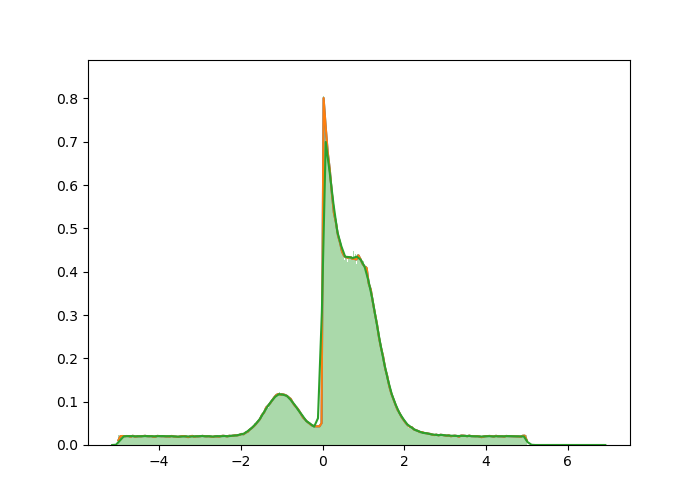
\includegraphics{plots/kde.png}
\caption{Kernel Density Estimation}\label{fig:kde}
}
\end{figure}

\[
\mathbf{r} \equiv \begin{bmatrix}
y \\
\theta
\end{bmatrix}
\] \{\#eq:eq1\}

\hypertarget{abstract-1}{%
\section{Abstract}\label{abstract-1}}

This study aims at comparing the speed and accuracy of differentu methods for one-dimensional kernel density estimation in Python/TensorFlow, especially concerning applications in high energy physics.

Starting from the basic algorithm, several optimizations from recent papers are introduced and combined to ameliorate the efficiency of the algorithm.

\hypertarget{literature}{%
\section{Literature}\label{literature}}

Here is a review of existing methods.

\hypertarget{methods-1}{%
\section{Methods}\label{methods-1}}

We describe our methods in this chapter.

\hypertarget{final-words}{%
\section{Final Words}\label{final-words}}

We have finished a nice book.


\listoftables
\listoffigures
\lstlistoflistings

\end{document}
